% header

\documentclass{beamer}
\usepackage[english]{babel}
\usepackage{amsmath,amssymb}
\usepackage[utf8]{inputenc}
\usetheme{Berkeley}

\usepackage{color}
\usepackage{xcolor}
\usepackage{listings}
\usepackage{url}
\usepackage[T1]{fontenc}
\usepackage{xspace}
\usepackage[style=iso]{datetime2}

\usepackage{tikz}
\usetikzlibrary{shapes.callouts,shadows, calc}
\usepackage{listings}


% Solarized colour scheme for listings
%
\definecolor{solarized@base03}{HTML}{002B36}
\definecolor{solarized@base02}{HTML}{073642}
\definecolor{solarized@base01}{HTML}{586e75}
\definecolor{solarized@base00}{HTML}{657b83}
\definecolor{solarized@base0}{HTML}{839496}
\definecolor{solarized@base1}{HTML}{93a1a1}
\definecolor{solarized@base2}{HTML}{EEE8D5}
\definecolor{solarized@base3}{HTML}{FDF6E3}
\definecolor{solarized@yellow}{HTML}{B58900}
\definecolor{solarized@orange}{HTML}{CB4B16}
\definecolor{solarized@red}{HTML}{DC322F}
\definecolor{solarized@magenta}{HTML}{D33682}
\definecolor{solarized@violet}{HTML}{6C71C4}
\definecolor{solarized@blue}{HTML}{268BD2}
\definecolor{solarized@cyan}{HTML}{2AA198}
\definecolor{solarized@green}{HTML}{859900}

% tikz listings support for highlighting - just insert backticks.
\tikzset{note/.style={rectangle callout, rounded corners,fill=gray!20,drop shadow,font=\footnotesize}}    

\newcommand{\tikzmark}[1]{\tikz[overlay,remember picture] \node (#1) {};}    

\newcounter{calloutcounter}
\setcounter{calloutcounter}{1}

\makeatletter
\newenvironment{btHighlight}[1][]
{\begingroup\tikzset{bt@Highlight@par/.style={#1}}\begin{lrbox}{\@tempboxa}}
{\end{lrbox}\bt@HL@box[bt@Highlight@par]{\@tempboxa}\endgroup}

\newcommand\btHL[1][]{%
  \begin{btHighlight}[#1]\bgroup\aftergroup\bt@HL@endenv%
}
\def\bt@HL@endenv{%
  \end{btHighlight}%   
  \egroup
}
\newcommand{\bt@HL@box}[2][]{%
  \tikz[#1]{%
    \pgfpathrectangle{\pgfpoint{0pt}{0pt}}{\pgfpoint{\wd #2}{\ht #2}}%
    \pgfusepath{use as bounding box}%
    \node[anchor=base west,rounded corners, fill=green!30,outer sep=0pt,inner xsep=0.2em, inner ysep=0.1em,  #1](a\thecalloutcounter){\usebox{#2}};
  }%
   %\tikzmark{a\thecalloutcounter} <= can be used, but it leads to a spacing problem
   % the best approach is to name the previous node with (a\thecalloutcounter)
 \stepcounter{calloutcounter}
}
\makeatother


\lstset{
  language=C++,
  basicstyle=\footnotesize\ttfamily,
  rangeprefix=//\ ,
  includerangemarker=false,
}

% Define C++ syntax highlighting colour scheme
\lstdefinelanguage{cpp}{
  language=C++,
  basicstyle=\footnotesize\ttfamily,
  numbers=left,
  numberstyle=\footnotesize,
  tabsize=2,
  breaklines=true,
  escapeinside={@}{@},
  numberstyle=\tiny\color{solarized@base01},
  keywordstyle=\color{solarized@green},
  stringstyle=\color{solarized@cyan}\ttfamily,
  identifierstyle=\color{solarized@blue},
  commentstyle=\color{solarized@base01},
  emphstyle=\color{solarized@red},
  frame=single,
  rulecolor=\color{solarized@base2},
  rulesepcolor=\color{solarized@base2},
  showstringspaces=false,
  moredelim={**[is][\btHL]{`}{`}},
}

\lstdefinelanguage{diff}{
  morecomment=[f][\color{blue}]{@@},           % group identifier
  morecomment=[f][\color{red}]{-},             % deleted lines
  morecomment=[f][\color{green!50!black}]{+},  % added lines
  morecomment=[f][\color{magenta}]{---},       % diff header lines
  morecomment=[f][\color{magenta}]{+++},
}

\lstdefinelanguage{plus}{
  basicstyle=\footnotesize\ttfamily\color{green!50!black},
  emph={see,below,TypeSwitch,unspecified},
  emphstyle=\itshape
}

\lstdefinelanguage{signature}{
  basicstyle=\ttfamily\color{green!50!black},
  emph={see,below,TypeSwitch,unspecified},
  emphstyle=\itshape
}

\newcommand{\desc}[1]{\textit{#1}}
\newcommand{\requires}{\desc{Requires}}
\newcommand{\effects}{\desc{Effects}}
\newcommand{\precondition}{\desc{Precondition}}
\newcommand{\postcondition}{\desc{Postcondition}}
\newcommand{\throws}{\desc{Throws}}
\newcommand{\returns}{\desc{Returns}}
\newcommand{\remarks}{\desc{Remarks}}
\newcommand{\exceptionsafety}{\desc{Exception Safety}}
\newcommand{\fullref}[1]{\ref{#1} \nameref{#1}}

\def\code#1{\texttt{#1}}
\newcommand\mypound{\protect\scalebox{0.8}{\raisebox{0.4ex}{\#}}}
\newcommand{\CC}{C\nolinebreak\hspace{-.05em}\raisebox{0.4ex}{\resizebox{!}{0.6\baselineskip}{\bf++}}}
\newcommand{\cplusplus}{\protect\CC\xspace}
\newcommand{\this}{\code{this}\xspace}
\newcommand{\self}{\code{self}\xspace}
\newcommand{\cvref}{\emph{cv-ref qualifiers}\xspace}
\newcommand{\nl}{\vspace{\baselineskip}}

\title{A Proper Property\\
       \cplusplus Gymnastics with Partially Defined Types}
\author{Gašper Ažman}
\date{November 27, 2017}


\begin{document}

\begin{frame}
  \titlepage
\end{frame}


\section{About: Author}
\begin{frame}
  \frametitle{About Me}
  \begin{itemize}
    \item Gašper Ažman
    \item Started teaching \cplusplus in highschool
    \item Did computer vision research at Berkeley
    \item Helped with Amazon Search Infrastructure at a9.com
    \item Currently at Citadel, building really cool research tools.
    \item A regular at the British Standards Insitute (BSI) Meetings
    \item On the programming committes of CppCon and C$++$Now.
  \end{itemize}
\end{frame}

\section{Disclaimer}

\begin{frame}
  \frametitle{Disclaimer}
  The opinions in this talk are my own, and do not necessarily reflect the
  opinions of Citadel LLC or any of its subsidiaries.\nl
  
  In addition, no Citadel resources were used in the development of this talk.
\end{frame}


\section{Recap}
\begin{frame}[fragile]
  \frametitle{So, What is a Property?}
  A property pretends to be a field.\nl
  
  Assignment:
  \begin{lstlisting}[language=cpp]
    airplane.cargo = 5;
  \end{lstlisting}

  Reading:
  \begin{lstlisting}[language=cpp]
    int x = airplane.cargo;
  \end{lstlisting}
\end{frame}


\begin{frame}[fragile]
  \frametitle{Totally.}
  If it quacks like a field, it has to be...
  
  \begin{lstlisting}[language=cpp]
    struct Airplane {
      int cargo;
    } airplane;
  \end{lstlisting}
  
  ... a field, right?
\end{frame}


\begin{frame}[fragile]
  \frametitle{Have you heard of this?}

  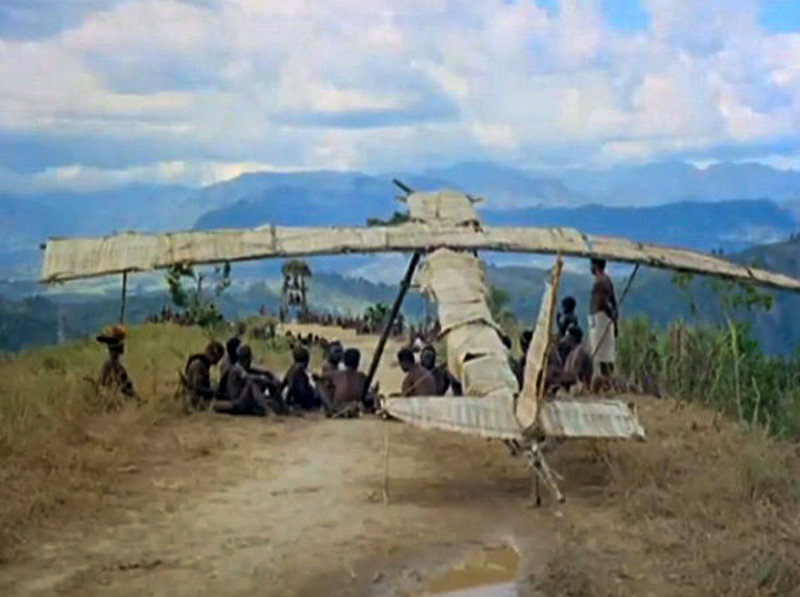
\includegraphics[width=\textwidth]{CargoCultAirplane.jpg}
\end{frame}


\begin{frame}[fragile]
  \frametitle{It is only a shell...}
 
  Instead, it's a pair of a Getter and a Setter.
  \begin{lstlisting}[language=cpp]
struct Airplane {
  struct Cargo {
    operator int() const { /* getter */
      return 0;
    }
    int operator=(int y) { /* setter */
      return 0;
    }
  };

  Cargo cargo;
} airplane;
  \end{lstlisting}
\end{frame}


\begin{frame}[fragile]
  \frametitle{Ta-Da! We're Done, right?}

  No. Need access to the Host's \code{this} pointer.
  \begin{lstlisting}[language=cpp]
template <typename Payload>
struct Airplane {
  bool cargo_loaded; // can't reload
  std::optional<Payload> private_cargo;
  struct Cargo {
    operator Payload() {
      return *std::exchange(`private_cargo`, {}};
    }
    void operator=(Payload package) {
      if (!`cargo_loaded`) {
        @@`cargo_loaded` = true;
        @@`private_cargo` = std::move(package);
      }
    }
  } cargo;
} airplane;
  \end{lstlisting}
\end{frame}

\end{document}
